\section{Modelado y propiedades ópticas}
\label{section:optical_properties}

Para modelar la morfología bicóncava característica de los eritrocitos, se han propuesto diversos enfoques analíticos, entre los que destacan los modelos de Skalak \cite{skalakStrainEnergyFunction1973}, Lu \cite{luSimulationsLightScattering2005}, Fung \cite{fungHighresolutionDataGeometry1981},
 y los óvalos de Cassini \cite{ereminaDifferentShapeModels2006a}. En este trabajo se emplea el modelo basado en óvalos de Cassini, debido a su simplicidad analítica y su capacidad para reproducir fielmente la morfología promedio de un eritrocito sano, optimizando el costo computacional en simulaciones de esparcimiento \cite{ereminaDifferentShapeModels2006a}. Los óvalos de Cassini son curvas planas definidas como el lugar geométrico de los puntos cuyo producto de distancias a dos focos fijos es constante; esto los distingue de las elipses, donde se conserva la suma de dichas distancias \cite{wriedtLightScatteringSingle2006a}. Al rotar un óvalo de Cassini alrededor de su eje de simetría, se genera un sólido de revolución con la geometría de un disco bicóncavo. En coordenadas cartesianas, asumiendo simetría axial respecto al eje $z$, la superficie se describe mediante la expresión \cite{ereminaDifferentShapeModels2006a}
 %
 \begin{tcolorbox}[ams align]
 	z(x) = \pm c \sqrt{-a^2 - x^2 \pm \sqrt{4x^2a^2 + b^4}},
 	\label{eq:cassini}
 \end{tcolorbox}
 %
donde los signos $\pm$ externos definen la simetría especular de las superficies superior e inferior, mientras que los internos delimitan las ramas del óvalo. Los parámetros geométricos se interpretan de la siguiente manera: $a$ representa la semidistancia focal, $b$ es la raíz cuadrada del producto constante de las distancias a los focos, y $c$ es un factor de escala que ajusta el espesor máximo \cite{wriedtLightScatteringSingle2006a}. La relación entre estos parámetros delimita la forma del eritrocito: un incremento en $a$ acentúa la depresión central (bicóncavidad), mientras que valores menores de $a$ derivan en geometrías convexas o incluso esferoidales. Por su parte, $b$ escala las dimensiones globales de la curva, controlando así el volumen total \cite{ereminaDifferentShapeModels2006a}. En la Fig. \ref{fig:Cassini_ovals} se muestra un modelo con parámetros $a=2.6$ $\mu$m, $b=2.7$ $\mu$m y $c=0.8$ $\mu$m, los cuales corresponden a un eritrocito sano con un volumen de $79.2$ $\mu$m$^3$. La Fig. \ref{subfig:bidimesional} muestra la sección transversal, mientras que la Fig. \ref{subfig:front} presenta el corte frontal del sólido de revolución resultante.
%
\begin{figure}[b]
	\centering
	\sidesubfloat[First image]{\hspace{-0.5cm}{
		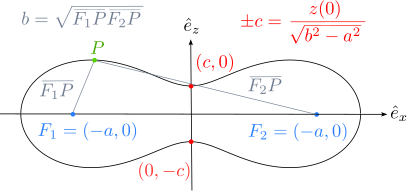
\includegraphics[width=0.35\textwidth]{../Figuras/Cassini.pdf}\label{subfig:bidimesional}}}\hspace{0.5cm}
	\sidesubfloat[Second image]{\hspace{-0.2cm}{	
\includegraphics[width=0.3\textwidth]{../Figuras/axial_ery.pdf}\label{subfig:front}}}
	\caption{Óvalo de Cassini con valores de $a=2.6\,\mu\text{m}, b=2.7\,\mu\text{m}$ y $c=0.8\,\mu\text{m}$ que representa a un eritrocito sano con volumen de $79.2\,\mu\text{m}^3$. \textbf{a)} Corte frontal del sólido de revolución resultante.}
	\label{fig:Cassini_ovals}
\end{figure}
%

La descripción morfológica proporcionada por los óvalos de Cassini define el dominio espacial ocupado por la partícula; no obstante, la respuesta electromagnética y, en particular, los procesos de esparcimiento y absorción de la luz, están determinados por el contraste entre las propiedades ópticas del eritrocito y las del plasma \cite{bosschaartLiteratureReviewNovel2014a}. En el caso de los eritrocitos, su función dieléctrica está dada por la hemoglobina, por lo que variaciones de la CHCM modifican la respuesta óptica efectiva de la célula \cite{bosschaartLiteratureReviewNovel2014a}. Experimentalmente, los valores del índice de refracción de la hemoglobina se han obtenido a partir de mediciones de transmitancia y reflectancia mediante el uso de esferas integradoras y técnicas espectroscópicas \cite{friebelDeterminationComplexRefractive2005a, meinkeOpticalPropertiesPlatelets2007a}. No obstante, la mayoría de los datos disponibles en la literatura para distintas concentraciones de hemoglobina se encuentran restringidos a ventanas espectrales finitas.

Los datos experimentales de la parte real e imaginaria del índice de refracción empleados en este trabajo corresponden a tres valores de la CHCM: 15.3 g/dL \cite{friebelDeterminationComplexRefractive2005a}, 28.7 g/dL \cite{friebelModelFunctionCalculate2006} y 30.6~g/dL~\cite{friebelDeterminationComplexRefractive2005a}. La parte real del índice de refracción para todas las concentraciones se reporta en términos de la relación \cite{friebelModelFunctionCalculate2006}
%
\begin{equation}
	n_{\text{Hb}}(\lambda,c_{\text{Hb}})=n_{\text{H}_{2}\text{O}}(\lambda)\,[\beta(\lambda)c_{\text{Hb}}+1],
	\label{eq:IR_eri}
\end{equation}
%
donde $n_{\text{H}_{2}\text{O}}(\lambda)$ es el índice de refracción del agua, $\beta(\lambda)$ es el incremento refractivo específico de la hemoglobina y $c_{\text{Hb}}$ es la concentración de hemoglobina. En la Fig. \ref{subfig:beta} se muestra la dependencia espectral de $\beta(\lambda)$, donde los puntos indican los datos experimentales y la línea continua una interpolación. En la región ultravioleta se observa dispersión anómala, mientras que en los intervalos 310–355 nm y 500–1100 nm las variaciones de $\beta$ no son significativas: la desviación estándar del promedio en dichos rangos es del orden de $3.6\times10^{-5}$, comparable con el error experimental reportado para mediciones a una longitud de onda dada \cite{friebelModelFunctionCalculate2006}. En la Fig. \ref{subfig:refrac} se presentan las curvas de la parte real del índice de refracción obtenidas a partir de la Ec.~\eqref{eq:IR_eri} para las distintas concentraciones: la curva verde para 15.3 g/dL, la roja para 28.7 g/dL y la azul para 30.6 g/dL. La curva gris punteada representa la parte real del índice de refracción del agua, incluida como referencia. La comparación entre las curvas correspondientes a distintas concentraciones de hemoglobina muestran la dependencia lineal
 de $n_{\text{Hb}}$ con $c_{\text{Hb}}$. En cuanto a la parte imaginaria, para la concentración de 28.7 g/dL se dispone de datos en el intervalo espectral de 250 a 1100 nm. En contraste, para las concentraciones de 15.3 g/dL y 30.6 g/dL la información experimental de la parte imaginaria sólo está disponible en el rango de 300 a 600 nm. Para el plasma, se emplearon los datos de la parte real reportados en \cite{liuMeasurementRefractiveIndex2019} y de la parte imaginaria en \cite{meinkeOpticalPropertiesPlatelets2007a}, ambos en el intervalo espectral comprendido entre 400 y 750 nm.
%
\begin{figure}[t]
	\centering
	\sidesubfloat[First image]{\hspace{-0.5cm}{
			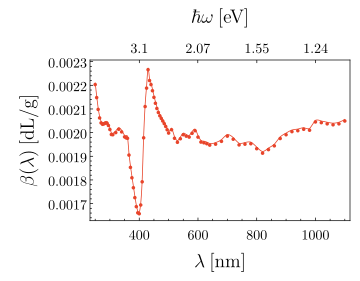
\includegraphics[width=0.48\textwidth]{../Figuras/beta.pdf}\label{subfig:beta}}}\hspace{0.1cm}
	\sidesubfloat[Second image]{\hspace{-0.4cm}{	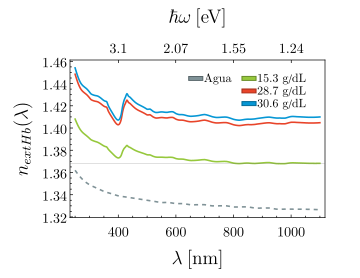
\includegraphics[width=0.457\textwidth]{../Figuras/refractive_index.pdf}\label{subfig:refrac}}}\vspace{-0.5cm}
	\caption{Datos empleados reportados en \cite{meinkeOpticalPropertiesPlatelets2007a} para el índice de refracción de la hemoglobina a distintas concentraciones. \textbf{a)} Incremento refractivo específico de la hemoglobina en términos de la longitud de onda. Los puntos rojos representan datos experimentales y la línea continua una interpolación. \textbf{b)} Parte real del índice de refracción de la hemoglobina para distintas concentraciones: 15.3 g/dL, 28.7 g/dL y 30.6 g/dL indicados mediante las líneas continuas verde, roja y azul, respectivamente. La línea gris punteada indica la parte real del índice de refracción del agua. }
	\label{fig:dataEri}
\end{figure}
%

Con el fin de disponer de una representación continua y analítica de la función dieléctrica en todo el rango del visible, la parte imaginaria de la función dieléctrica de los eritrocitos y del plasma se ajustó mediante un modelo de osciladores de Lorentz\footnote{En este modelo, los electrones del material se describen como osciladores armónicos amortiguados con frecuencias de resonancia características, sometidos a la acción de un campo electromagnético externo \cite{bohrenAbsorptionScatteringLight2008a}.}. Esta elección, aunque no es única, resulta particularmente conveniente porque proporciona una expresión analítica que, por construcción, satisface el principio de causalidad \cite{maggioreModernIntroductionClassical2023} y, por lo tanto, es compatible con las relaciones de KK. El ajuste se realizó por mínimos cuadrados entre los datos experimentales y el modelo propuesto, empleando un número finito de osciladores (véase el Apéndice \ref{section:apendix1}). En la Fig.~\ref{subfig:ajuste_ery} se muestran los datos experimentales correspondientes a la parte imaginaria de la función dieléctrica de eritrocitos con una CHCM de 28.7 g/dL, extraídos de \cite{friebelDeterminationComplexRefractive2005a} (puntos rojos), junto con el ajuste obtenido mediante osciladores de Lorentz (línea azul continua). De manera análoga, en la Fig.~\ref{subfig:ajuste_plasma} se presentan los datos experimentales de la parte imaginaria de la función dieléctrica del plasma (puntos rojos) y su correspondiente ajuste mediante osciladores de Lorentz (línea azul continua). En ambos casos, las líneas grises verticales indican las frecuencias de resonancia asociadas a los osciladores empleados.
%
\begin{figure}[h!]
	\centering
	\sidesubfloat[First image]{\hspace{-0.8cm}{
		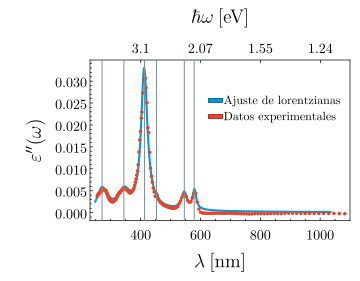
\includegraphics[width=0.47\textwidth]{../Figuras/ajusteLorentz28.pdf}\label{subfig:ajuste_ery}}}\hspace{0.1cm}
	\sidesubfloat[Second image]{\hspace{-0.5cm}{	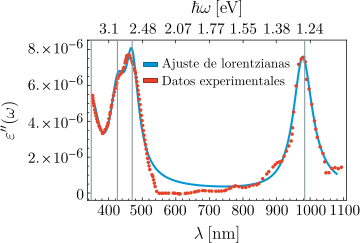
\includegraphics[width=0.51\textwidth]{../Figuras/ajustePlasma.pdf}\label{subfig:ajuste_plasma}}}\vspace{-0.7cm}
	\caption{Parte imaginaria de la función dieléctrica. \textbf{a)} Función dieléctrica de eritrocitos con una concentración de 28.7 g/dL. Los datos experimentales se obtuvieron de \cite{friebelModelFunctionCalculate2006} y están indicados mediante puntos rojos. La línea azul continua representa el ajuste con lorentzianas obtenido.  \textbf{b)} Función dieléctrica del plasma, cuyos datos experimentales representados por puntos rojos se extrajeron de \cite{meinkeOpticalPropertiesPlatelets2007a}. La línea azul continua reperesenta el ajuste con lorentzianas obtenido. En ambas figuras las líneas grises verticales indican las frecuencias de resonancia asociadas a los osciladores de Lorentz empleados en el ajuste.}
	\label{fig:ajuste}
\end{figure}
%

Dado que los datos experimentales disponibles cubren únicamente ventanas espectrales finitas, los ajustes con lorentzianas no incorporan de manera explícita las contribuciones asociadas a transiciones electrónicas situadas fuera de dichos intervalos. En consecuencia, la aplicación directa de las relaciones de KK a estos espectros truncados conduciría a inconsistencias entre las partes real e imaginaria de la función dieléctrica. Para mitigar este problema se emplearon las relaciones SSKK, las cuales introducen una frecuencia de anclaje que permite reducir los errores asociados al truncamiento espectral \cite{KramersKronigRelationsOptical2005}. En este trabajo la frecuencia de anclaje se determinó mediante un ajuste por mínimos cuadrados entre la parte real experimental de la función dieléctrica y la obtenida a partir de las relaciones SSKK (ver Apéndice \ref{section:apendix2}), obteniéndose valores de 3.59 eV, 3.41 eV y 3.39 eV para las concentraciones de hemoglobina de 15.3 g/dL, 28.7 g/dL y 30.6 g/dL, respectivamente, y de 2.39 eV para el plasma. En la Fig. \ref{subfig:epsSSKK_eri} se muestra la comparación entre la parte real de la función dieléctrica reconstruida mediante SSKK, indicada mediante la línea azul continua, y los datos experimentales para una CHCM de 28.7 g/dL indicados mediante los puntos rojos, observándose una desviación promedio de 0.003. De manera análoga, la Fig. \ref{subfig:epsSSKK_Plasma} muestra la parte real de la función dieléctrica obtenida mediante el análisis de SSKK como una línea azul continua, donde se observa una desviación promedio de 0.015 respecto a los datos experimentales (puntos rojos). Esta diferencia, particularmente en el ultravioleta se debe a que se ha reportado que el índice de refracción de soluciones de hemoglobina y del plasma presenta un incremento pronunciado en el ultravioleta profundo, asociado principalmente a la absorción del agua \cite{bosschaartLiteratureReviewNovel2014a}.  Este comportamiento no se reproduce completamente en el presente análisis, ya que los espectros de absorción disponibles para la hemoglobina y el plasma —y, por ende, la parte imaginaria de la función dieléctrica empleada— sólo se extienden hasta aproximadamente 250 nm y 300 nm, respectivamente.  Aun con esta limitación, el uso de SSKK permite obtener una reconstrucción con un error promedio casi siete veces menor que el reportado en \cite{bosschaartLiteratureReviewNovel2014a}, donde se emplean únicamente las relaciones de KK estándar. En principio, la extensión de los datos experimentales a un rango espectral más amplio \cite{KramersKronigRelationsOptical2005} o el uso de múltiples frecuencias de anclaje mediante relaciones MSKK\footnote{Las relaciones de Kramers–Kronig generalizadas con sustracciones múltiples (MSKK) permiten introducir varias frecuencias de anclaje para mejorar la precisión del análisis \cite{palmerMultiplySubtractiveKramers1998}.} permitiría mejorar la reconstrucción de la función dieléctrica en la región ultravioleta.
%
\begin{figure}[bt]
	\centering
	\sidesubfloat[First image]{\hspace{-0.8cm}{
			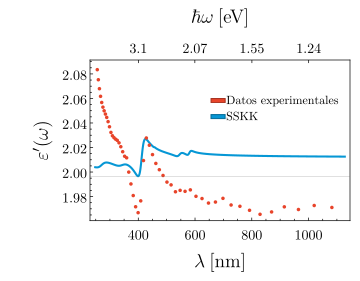
\includegraphics[width=0.47\textwidth]{../Figuras/sskk28.pdf}\label{subfig:epsSSKK_eri}}}\hspace{0.1cm}
	\sidesubfloat[Second image]{\hspace{-0.6cm}{	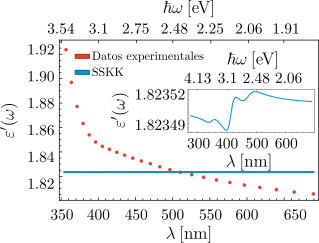
\includegraphics[width=0.52\textwidth]{../Figuras/sskkPlasma1.pdf}\label{subfig:epsSSKK_Plasma}}}\vspace{-0.7cm}
	\caption{Comparación entre la parte real de la función dieléctrica reconstruida mediante las relaciones SSKK (línea azul continua) y los datos experimentales (puntos rojos) para: \textbf{a)} eritrocitos con una CHCM de 28.7 g/dL, a partir de los datos reportados en \cite{friebelModelFunctionCalculate2006}; y \textbf{b)} plasma, empleando los datos experimentales de \cite{meinkeOpticalPropertiesPlatelets2007a}.}
	\label{fig:epsSSKK}
\end{figure}
%

Cabe destacar que, aunque para la concentración de 28.7 g/dL se dispone de datos experimentales tanto de la parte real como de la imaginaria en un intervalo espectral relativamente amplio, en este trabajo se empleó de manera consistente la función dieléctrica reconstruida mediante el mismo procedimiento (ajuste con osciladores de Lorentz seguido de SSKK) para las tres concentraciones consideradas. Esta elección garantiza que todas las funciones dieléctricas estén sujetas a los mismos efectos de truncamiento espectral, de modo que las comparaciones posteriores de las propiedades ópticas calculadas reflejen exclusivamente la variación de la CHCM y no diferencias metodológicas en el tratamiento de los datos.

En la Fig.~\ref{fig:epsEri} se muestran las partes real [Fig. \ref{subfig:epsReEri}] e imaginaria [Fig. \ref{subfig:epsImEri}] de la función dieléctrica para las distintas concentraciones de hemoglobina consideradas: verde para 15.3 g/dL, rojo para 28.7 g/dL y azul para 30.6 g/dL. En todas las curvas destaca, en el ultravioleta–visible cercano, la banda de Soret, característica de la hemoglobina, con un máximo situado típicamente en el intervalo 410–430 nm \cite{bosschaartLiteratureReviewNovel2014a}, cuya intensidad es considerablemente mayor que la de las transiciones en el visible. En esta última región se observan las denominadas bandas Q, correspondientes a la banda $\alpha$ (a mayor longitud de onda) y la banda $\beta$ (a menor longitud de onda), cuyos máximos se localizan de manera general en los rangos aproximados 600–650 nm y 520–580 nm \cite{dayerBandAssignmentHemoglobin2010}, respectivamente, dependiendo de la concentración y del estado de oxigenación\footnote{Estas bandas se originan en transiciones electrónicas $\pi \rightarrow \pi^*$ del anillo de porfirina. Tanto la banda de Soret (UV–visible cercano) como las bandas Q (visible) son sensibles al estado de oxidación del hierro y a cambios conformacionales de la hemoglobina, por lo que caracterizan su estructura y función \cite{dayerBandAssignmentHemoglobin2010}.}. Las regiones sombreadas señalan las bandas espectrales mencionadas anteriormente. De manera adicional, tanto en la parte real como en la imaginaria se aprecia un relieve alrededor de 450 nm, que coincide con el flanco de la banda de Soret y marca la transición entre el régimen de dispersión anómala en el ultravioleta–visible cercano y el comportamiento más suave característico del visible.
%
\begin{figure}[th]
	\centering
	\sidesubfloat[First image]{\hspace{-0.8cm}{
			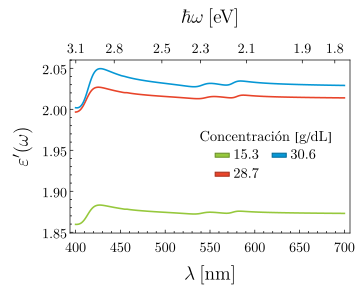
\includegraphics[width=0.48\textwidth]{../Figuras/parteReEri.pdf}\label{subfig:epsReEri}}}\hspace{0.1cm}
	\sidesubfloat[Second image]{\hspace{-0.4cm}{	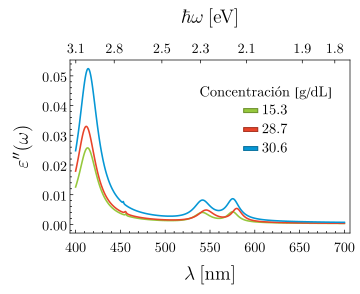
\includegraphics[width=0.48\textwidth]{../Figuras/parteImEri.pdf}\label{subfig:epsImEri}}}
	\caption{Función dieléctrica de eritrocitos para distintas concentraciones de hemoglobina, indicadas mediante líneas continuas verde, roja y azul correspondientes a 15.3 g/dL, 28.7 g/dL y 30.6 g/dL, respectivamente. Las regiones sombreadas señalan las bandas espectrales que dominan la respuesta óptica de los eritrocitos en el ultravioleta y el visible. \textbf{a)} Parte real de la función dieléctrica. \textbf{b)} Parte imaginaria de la función dieléctrica.}
	\label{fig:epsEri}
\end{figure}
%
